% -------------------------------------------------
% Capítulo: Metodología de gestión del proyecto
% Orden del director (19-sep-2026): metodología para mover los tickets, pantallazo del
% tablero, criterios de aceptación, Definition of Ready y Definition of Done.
% Cifras del tablero tomadas de GitHub Projects el 25-sep-2026 (gh project item-list).
% -------------------------------------------------

Este capítulo describe cómo se gestionó el trabajo de desarrollo: la herramienta y el flujo con que se movieron las tareas, los criterios con que una tarea se consideraba lista para empezar y terminada, y los criterios de aceptación de los requerimientos.

\section{Enfoque de trabajo}
\label{sec:ges_enfoque}

El anteproyecto planteó un enfoque ágil inspirado en Scrum (Capítulo 4). En la práctica, al ser un proyecto con un solo desarrollador, las ceremonias de Scrum pensadas para equipos (planeación de \textit{sprint}, reunión diaria, retrospectiva grupal) se simplificaron y el trabajo se gestionó con un tablero Kanban \cite{kanban_method}: las tareas avanzan por columnas a medida que cambian de estado, y el ritmo lo marcaron las reuniones de seguimiento con el director del trabajo de grado, en las que se revisaba el avance y se acordaban los siguientes pasos.

\section{Tablero en GitHub Projects}
\label{sec:ges_tablero}

Las tareas se registraron en GitHub Projects \cite{github_projects}, en el proyecto ``Gestor de Inventario de Materia Prima con Módulo LLM'', vinculado al repositorio del código. El tablero tiene cinco columnas:

\begin{itemize}
    \item \textbf{Backlog}: tareas identificadas que aún no se han preparado para empezar.
    \item \textbf{Ready}: tareas que cumplen la \textit{Definition of Ready} y pueden tomarse.
    \item \textbf{In progress}: tareas en desarrollo.
    \item \textbf{In review}: tareas terminadas en código que se están verificando.
    \item \textbf{Done}: tareas que cumplen la \textit{Definition of Done}.
\end{itemize}

Al 25 de septiembre de 2026 el proyecto contaba con 130 tareas: 75 en \textit{Done}, 3 en \textit{Ready} y 52 en \textit{Backlog}. Buena parte de las tareas del \textit{Backlog} corresponden a mejoras identificadas al comparar el sistema con productos comerciales, que quedaron fuera del alcance de este trabajo (Capítulo 13). La Figura \ref{fig:ges_tablero} muestra la vista de tablero.

\begin{figure}[H]
\centering
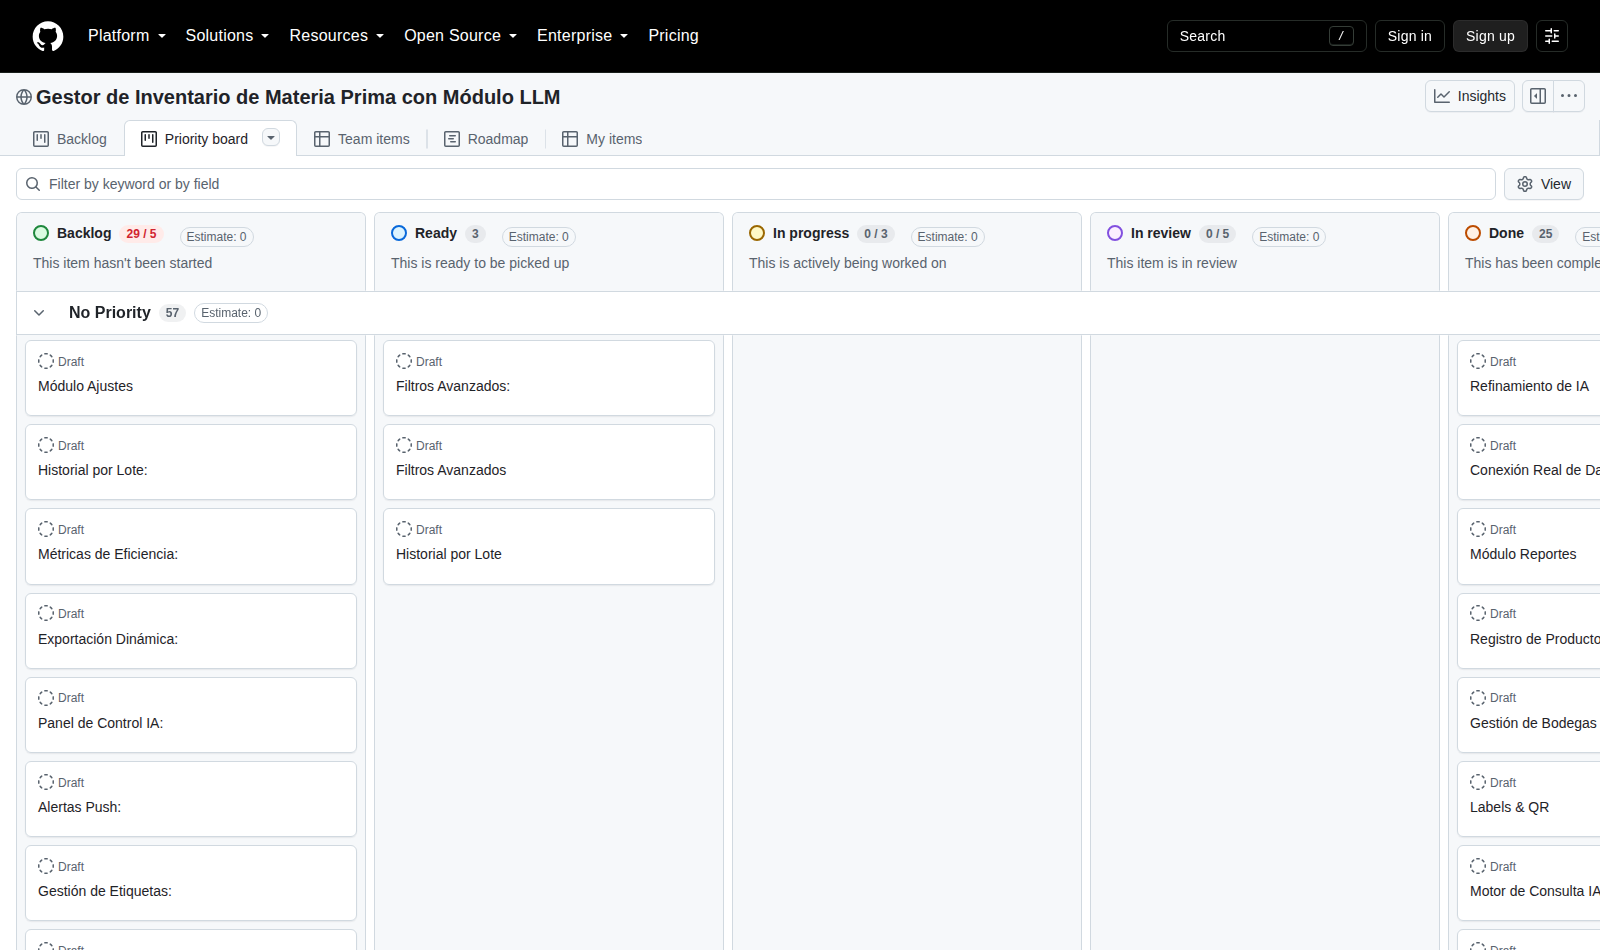
\includegraphics[width=\textwidth]{Imagenes/github_project_board.png}
\caption{Tablero del proyecto en GitHub Projects (vista \textit{Priority board}, 25 de septiembre de 2026).}
\label{fig:ges_tablero}
\end{figure}

\section{Flujo de una tarea}
\label{sec:ges_flujo}

Cada tarea recorrió el mismo camino:

\begin{enumerate}
    \item Se registra en \textit{Backlog} con un título que describe el resultado esperado; cuando corresponde a un requerimiento, se indica su identificador (por ejemplo, \texttt{[RNF-01]}).
    \item Cuando cumple la \textit{Definition of Ready}, pasa a \textit{Ready}.
    \item Al empezar a trabajarla pasa a \textit{In progress}; el trabajo se hace en el repositorio con commits descriptivos.
    \item Con el código terminado pasa a \textit{In review}: se ejecutan las pruebas automatizadas y se verifica manualmente el comportamiento.
    \item Cuando cumple la \textit{Definition of Done} pasa a \textit{Done}.
\end{enumerate}

\section{Criterios de aceptación}
\label{sec:ges_aceptacion}

Una tarea se aceptaba cuando cumplía los criterios de aceptación del requerimiento que implementaba. Los criterios se expresan en la forma \textit{dado / cuando / entonces}, y los principales están respaldados por una prueba automatizada (Capítulo \ref{chap:pruebas}). La Tabla \ref{tab:ges_criterios} muestra ejemplos para las reglas de negocio de la dirección.

\begin{longtable}{|p{1.4cm}|p{9.6cm}|p{3.6cm}|}
\caption{Ejemplos de criterios de aceptación y la prueba que los verifica.}
\label{tab:ges_criterios}\\
\hline
\textbf{RF} & \textbf{Criterio de aceptación} & \textbf{Prueba} \\
\hline
\endfirsthead
\hline
\textbf{RF} & \textbf{Criterio de aceptación} & \textbf{Prueba} \\
\hline
\endhead
RF-04 & \textbf{Dado} un material con dos lotes activos que vencen en fechas distintas, \textbf{cuando} se consume una cantidad, \textbf{entonces} se descuenta primero del lote que vence primero. & \texttt{ConsumptionFefoTest}, \texttt{FefoTest} \\ \hline
RF-05 & \textbf{Dado} un movimiento registrado en el Kardex, \textbf{cuando} alguien intenta modificarlo o eliminarlo, \textbf{entonces} el sistema lo rechaza y el registro permanece igual. & \texttt{KardexInmutableTest} \\ \hline
RF-06 & \textbf{Dado} un usuario con rol operario, \textbf{cuando} intenta gestionar usuarios o claves de API, \textbf{entonces} recibe acceso denegado (HTTP 403). & \texttt{UserManagementTest} \\ \hline
RF-08 & \textbf{Dado} un umbral de días configurado por el administrador, \textbf{cuando} un lote vence dentro de ese umbral, \textbf{entonces} aparece como crítico en el tablero y en el inventario. & \texttt{FefoUmbralTest} \\ \hline
RF-12 & \textbf{Dado} un material que no está registrado, \textbf{cuando} se pregunta por él al asistente, \textbf{entonces} la respuesta indica que no está registrado y no muestra lotes de otros materiales. & \texttt{ChatRagContextTest} \\ \hline
\end{longtable}

\section{Definition of Ready y Definition of Done}
\label{sec:ges_dor_dod}

La \textit{Definition of Ready} (DoR) establece cuándo una tarea está lista para empezar, y la \textit{Definition of Done} (DoD) cuándo puede darse por terminada. En un equipo, la DoD suele exigir pruebas unitarias y de integración, revisión del código por otra persona y despliegue; aquí había un solo desarrollador, que además probaba, así que no hubo revisión por pares. Los criterios aplicados en la práctica fueron:

\textbf{Definition of Ready.} Una tarea pasa a \textit{Ready} cuando:
\begin{itemize}
    \item su título describe el resultado esperado, no la actividad;
    \item está asociada a un requerimiento o a una observación de la dirección;
    \item tiene al menos un criterio de aceptación verificable;
    \item no depende de otra tarea sin terminar; y
    \item es lo bastante pequeña para completarse entre dos reuniones de seguimiento.
\end{itemize}

\textbf{Definition of Done.} Una tarea pasa a \textit{Done} cuando:
\begin{itemize}
    \item las pruebas unitarias y de integración (PHPUnit) pasan, incluidas las nuevas que cubren el cambio;
    \item se hicieron pruebas manuales del comportamiento en el navegador;
    \item el cambio está en la rama principal del repositorio en GitHub y el flujo de integración continua terminó sin errores; y
    \item el cambio está desplegado en producción (\url{https://app.pymetory.com}) y se verificó que funciona allí.
\end{itemize}

Desplegar directamente a producción, sin entorno intermedio, no es la práctica habitual; aquí el riesgo se redujo porque la integración continua detiene el despliegue si una prueba falla, se respaldó la base de datos antes de la migración que modificó el Kardex y cada despliegue se verifica en producción antes de cerrar la tarea.
